\begin{enumerate}[label=\thesection.\arabic*.,ref=\thesection.\theenumi]
\numberwithin{equation}{enumi}
\numberwithin{figure}{enumi}
%%
\item
\label{ch4_sim}
Plot 
\begin{equation}
P_e = \pr{\hat{X} = -1|X=1}
\end{equation}
%
for 
\begin{equation}
Y = AX+N,
\end{equation}
where $A$ is Raleigh with $E\sbrak{A^2} = \gamma, N \sim \gauss{0}{1}, X \in \brak{-1,1}$ for $0 \le \gamma \le 10$ dB.
\\
\solution See Fig. \ref{fig:probman_p_e_gamma}

%
\item
Assuming that $N$ is a constant, find an expression for $P_e$.  Call this $P_e(N)$.
\\
\solution The estimated value $\hat{X}$ is given by
\begin{align}
\hat{X} = 
\begin{cases}
+1 & Y>0\\
-1 & Y<0
\end{cases}
\end{align}
For $X = 1$, 
\begin{align}
Y &= A + N\\
P_e &= \pr{\hat{X} = -1|X=1} \\
&= \pr{Y<0 |X=1}\\
&= \pr{A<-N}\\
&= F_A(-N)\\
&= \int_{-\infty}^{-N} f_A(x)dx
\end{align}
By definition
\begin{align}
f_A(x) = 
\begin{cases}
\frac{x}{\sigma^2}\exp\brak{{-\frac{x^2}{2\sigma^2}}} & x\geq0\\
0 & otherwise
\end{cases}
\end{align}
If $N>0, f_A(x) = 0$. Then,
\begin{align}
 P_e=0  
\end{align}
If $N<0$. Then,
\begin{align}
 P_e(N) &=\int_{-\infty}^{-N} f_A(x)dx\\
 &=\int_{-\infty}^{0} 0dx+\int_{0}^{-N} f_A(x)dx\\
 &=\int_{0}^{-N} \frac{x}{\sigma^2}\exp\brak{{-\frac{x^2}{2\sigma^2}}}dx\\
 &=1-\exp{\brak{-\frac{N^2}{2\sigma^2}}}
\end{align}
Therefore,
\begin{align}\label{pe(N)}
P_e(N) = 
\begin{cases}
1-\exp\brak{{-\frac{N^2}{2\sigma^2}}} & N<0\\
0 & otherwise
\end{cases}
\end{align}
%

%
\item
%
\label{ch4_anal}
For a function $g$,
\begin{equation}
E\sbrak{g(X)} = \int_{-\infty}^{\infty}g(x)p_{X}(x)\, dx
\end{equation}
%
Find $P_e = E\sbrak{P_e(N)}$.
\\
\solution
Since $N \sim \gauss{0}{1}$ ,
\begin{align}
  p_N(x)= \frac{1}{\sqrt{2\pi}}\exp \brak{-\frac{x^2}{2} }\\
\end{align}
And from \eqref{pe(N)} 
\begin{align}
    P_e(x)=
    \begin{cases}
1-\exp\brak{{-\frac{x^2}{2\sigma^2}}} & x<0\\
0 & otherwise
\end{cases}
\end{align}

\begin{align}
 P_e=E\sbrak{P_e(N)} = \int_{-\infty}^{\infty}P_e(x)p_{N}(x)\, dx  
\end{align}
If $x<0, P_e(x)=0$ and using the fact that for an even function
\begin{align}
\int_{-\infty}^{\infty}f(x)=2\int_{-\infty}^{0}f(x)   
\end{align}
we get
\begin{align}
  P_e&= \frac{1}{\sqrt{2\pi}}\int_{-\infty}^{0}\exp \brak{ -\frac{x^2}{2}} \brak{1-\exp \brak{ -\frac{x^2}{2\sigma^2}} } dx\\
&= \frac{1}{2\sqrt{2\pi}} \int_{-\infty}^{\infty} \exp \brak{ -\frac{x^2}{2} }dx \nonumber \\
&- \frac{1}{2\sqrt{2\pi}} \int_{-\infty}^{\infty} \exp \brak{-\frac{(1+ \sigma^2)x^2}{2 \sigma^2}}  dx\\
&= \frac{\sqrt{2\pi} - \sqrt{\frac{\pi(2\sigma^2)}{1+\sigma^2}}}{2\sqrt{2\pi}}\\
&= \frac{1}{2} - \frac{1}{2}\sqrt{\frac{\sigma^2}{1+\sigma^2}}
\end{align}
For a Rayleigh Distribution with scale $= \sigma$,
\begin{align}
E\sbrak{A^2} = 2\sigma^2\\
\gamma = 2\sigma^2\\
\therefore P_e = \frac{1}{2} - \frac{1}{2}\sqrt{\frac{\gamma}{2+\gamma}}
\end{align}
%
%
\item
Plot $P_e$ in problems \ref{ch4_sim} and \ref{ch4_anal} on the same graph w.r.t $\gamma$.  Comment.
\\
\solution $P_e$ is plotted w.r.t $\gamma$ in \ref{fig:probman_p_e_gamma} using the code below.
\begin{lstlisting}
codes/cond/7.4.py
\end{lstlisting}
\begin{figure}[!ht]
\centering
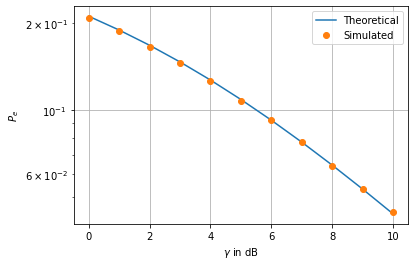
\includegraphics[width=\columnwidth]{figs/cond/7.4.png}
\caption{$P_e$ w.r.t $\gamma$}
\label{fig:probman_p_e_gamma}
\end{figure}
%
\end{enumerate}
